\subsection[Trasformare le distribuzioni]{Trasformare le distribuzioni}

\begin{frame}
	
	\frametitle{{\color{GradientDescentDiagramOrange}Trasformare le distribuzioni}}
	
	
	%In clustering, you calculate the similarity between two examples by combining all the feature data for those examples into a numeric value. Combining feature data requires that the data have the same scale. This section looks at normalizing, transforming, and creating quantiles, and discusses why quantiles are the best default choice for transforming any data distribution. Having a default choice lets you transform your data without inspecting the data's distribution.
	
	%\begin{block}{}
		Partiamo da un esempio: nel clustering, si calcola la similarità/dissimilarità tra due esempi prendendo in considerazione tutte le features numeriche.
		Utilizzando le features numeriche per utilizzare una metrica tra gli esempi è necessario che i dati siano nella stessa scala.
		\newlinedouble
		Il clustering è solo un esempio, molti altri algoritmi di apprendimento automatico richiedono che queste condizioni di scala nei dati utilizzati siano verificate al fine di funzionare efficientemente.
		\newlinedouble
		Esaminiamo quindi le operazioni più comuni applicate prima procedere con l'esecuzione degli algoritmi di apprendimento automatico:
		\begin{itemize}
			\item {\color{GradientDescentDiagramBlue}normalizzazione}
			\item {\color{GradientDescentDiagramRed}log-transform}
			\item {\color{GradientDescentDiagramGreen}quantili}
		\end{itemize}
	%\end{block}
	
\end{frame}





\subsubsection[Normalizzazione]{Normalizzazione}
\begin{frame}
	
	\frametitle{{\color{GradientDescentDiagramOrange}Trasformare le distribuzioni}: {\color{GradientDescentDiagramBlue}normalizzazione}}
	
	%\begin{block}{}
		È possibile trasformare i dati per più features nella stessa scala normalizzando i dati.
		In particolare, la normalizzazione è adatta per elaborare la distribuzione dei dati più comune, la \textbf{distribuzione gaussiana}.
		Rispetto ai quantili, la normalizzazione richiede un numero significativamente inferiore di dati per il calcolo.
		\newlinedouble
		Possiamo normalizzare i dati calcolando il relativo \textbf{z-score} come segue:
		\begin{empheq}[box=\fcolorbox{blue!40!black!60}{yellow!10}]{align*}
		x' = \frac{(x-\mu)}{\sigma} \quad:\quad\mu = \text{mean},\text{ }\sigma = \text{standard deviation}
		\end{empheq}
		
	%\end{block}
	
\end{frame}


\begin{frame}
	
	\frametitle{{\color{GradientDescentDiagramOrange}Trasformare le distribuzioni}: {\color{GradientDescentDiagramBlue}normalizzazione}}
	
	%\begin{block}{}
		Diamo un'occhiata alla somiglianza tra esempi normalizzati e non.	 Dalla figura mostrata sembrerebbe che il rosso è più simile al blu che al giallo.\\
		Tuttavia, le features sugli assi $x$ e $y$ \textbf{non hanno la stessa scala}.
		%Pertanto, la somiglianza osservata potrebbe essere legata al fatto che i dati non sono scalati.
		\newlinedouble
		Dopo la normalizzazione, tutte le features hanno la stessa scala; adesso in effetti il rosso è più simile al giallo. Pertanto, dopo aver normalizzato i dati, è possibile calcolare la somiglianza in modo più accurato.
		
		\begin{figure}[!htbp]
			\centering
			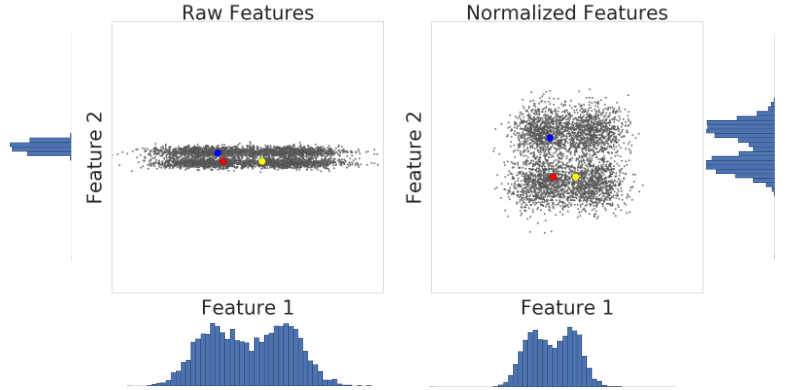
\includegraphics[width=8.0cm]{images/data_prep/scaling_distributions/NormalizeData.png}
					%\caption{Stripe Radar for Fraud Detection}
		\end{figure}
		
	%\end{block}
	
\end{frame}


\begin{frame}
	
	\frametitle{{\color{GradientDescentDiagramOrange}Trasformare le distribuzioni}: {\color{GradientDescentDiagramBlue}normalizzazione}}
	
	\begin{block}{Quando è opportuno normalizzare?}
		In sintesi, è opportuno applicare la normalizzazione quando una delle seguenti condizioni risulta verificata:
		\begin{itemize}
			\item i tuoi dati hanno una distribuzione gaussiana
			\item il tuo dataset non dispone di dati sufficienti per creare quantili
		\end{itemize}
	\end{block}
	
	\begin{block}{La normalizzazione min-max}
		Abbiamo visto la cosiddetta \textbf{normalizzazione z-score}, tuttavia a volte si preferisce utilizzare un'altro tipo di normalizzazione, più semplice, detta \textbf{normalizzazione min-max}:
		\begin{empheq}[box=\fcolorbox{blue!40!black!60}{yellow!10}]{align*}
		x' = \frac{x-min}{max-min} \quad:\quad min = \underset{\forall i \in D}{min}\text{ }x_i,\text{ }max = \underset{\forall i \in D}{max}\text{ }x_i
		\end{empheq}
	\end{block}
	
\end{frame}

\subsubsection[Log-Transform]{Log-Transform}
\begin{frame}
	
	\frametitle{{\color{GradientDescentDiagramOrange}Trasformare le distribuzioni}: {\color{GradientDescentDiagramRed}log-transform}}
		
	%\begin{block}{Quando è necessario normalizzare?}
		A volte, un dataset è conforme alla distribuzione \textbf{power law} ($f(x) = ax^k + o(x^k), \ x \to 0$) che raggruppa i dati all'estremità inferiore.\\
		%Nella figura, il rosso è più vicino al giallo che al blu.
		\begin{figure}[!htbp]
			\centering
			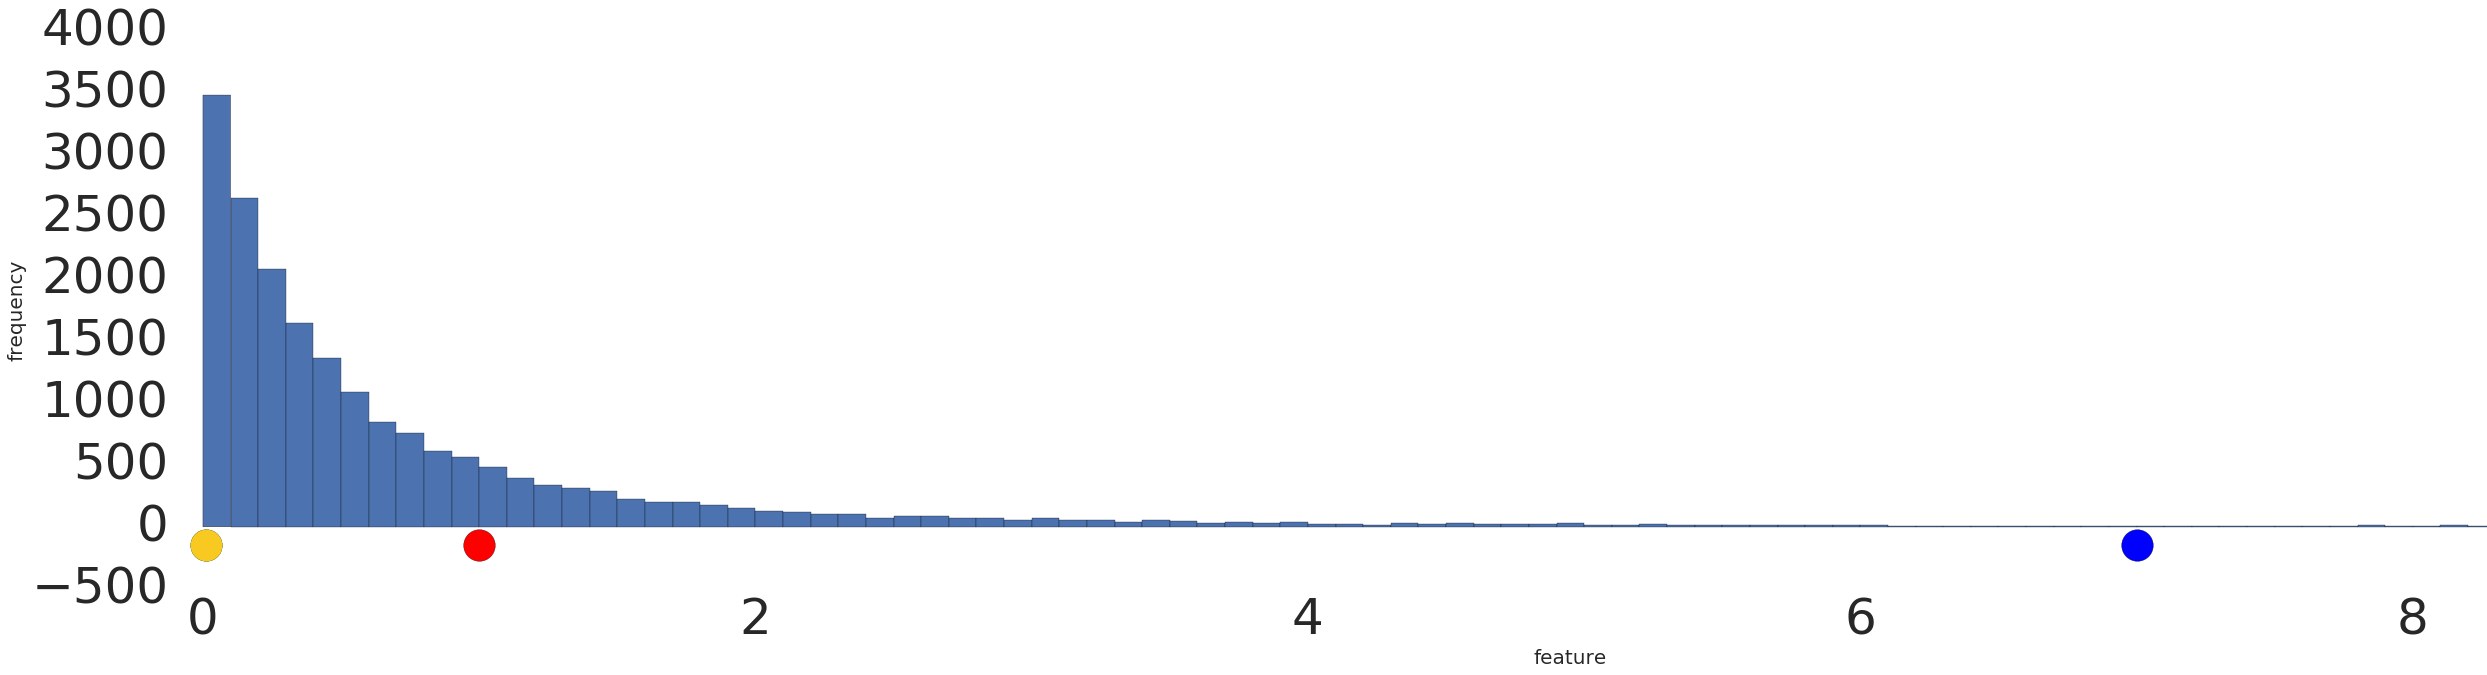
\includegraphics[width=8.0cm]{images/data_prep/scaling_distributions/LeftSkew.png}
					%\caption{Stripe Radar for Fraud Detection}
		\end{figure}
		
		Processiamo una distribuzione \textbf{power law} utilizzando una trasformazione logaritmica.
		Nella figura, la trasformazione logaritmica crea una distribuzione più uniforme. \textit{Notare la posizione dei punti tra prima e dopo}.
		% e il rosso è più vicino al blu che al giallo.
		
		\begin{figure}[!htbp]
			\centering
			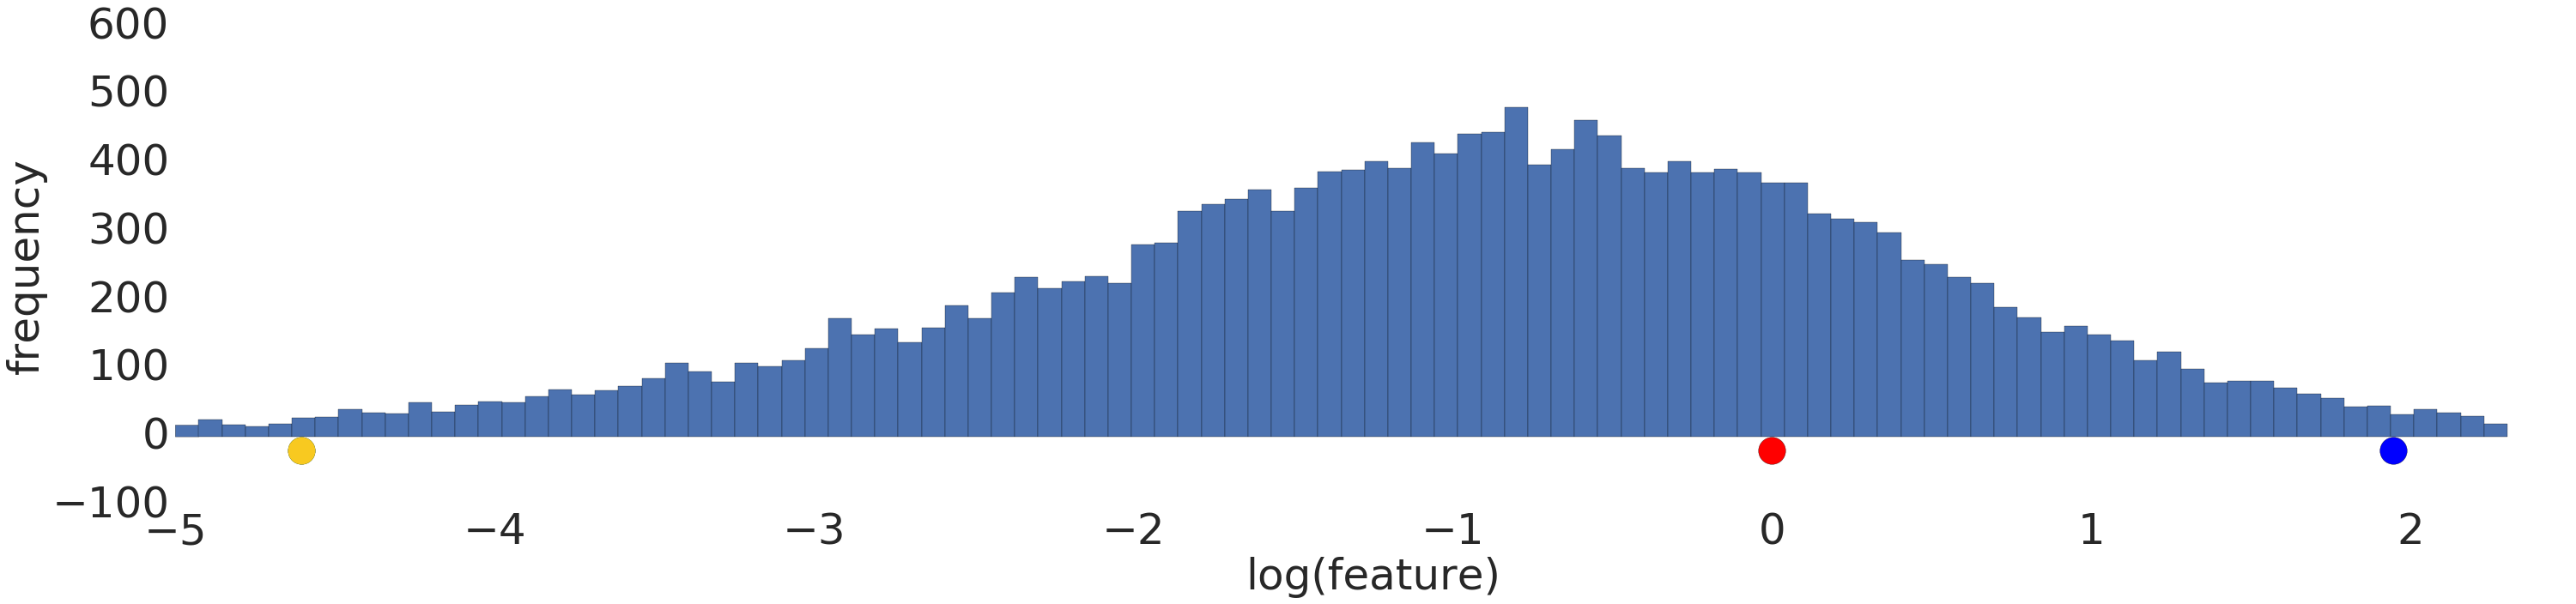
\includegraphics[width=8.0cm]{images/data_prep/scaling_distributions/NormalDistribution.png}
					%\caption{Stripe Radar for Fraud Detection}
		\end{figure}
	%\end{block}
	
\end{frame}

\subsubsection[Quantili]{Quantili}
\begin{frame}
	
	\frametitle{{\color{GradientDescentDiagramOrange}Trasformare le distribuzioni}: {\color{GradientDescentDiagramGreen}quantili}}
		
	%\begin{block}{}
		La normalizzazione e la log-transform riguardano distribuzioni di dati specifiche.\\
		Cosa succede se i dati non sono conformi a una distribuzione gaussiana o ad una legge di potenza?\\
		Esiste un \textbf{approccio generale} che si applica a qualsiasi distribuzione di dati? Proviamo a preprocessare questa distribuzione.
		
		\begin{figure}[!htbp]
			\centering
			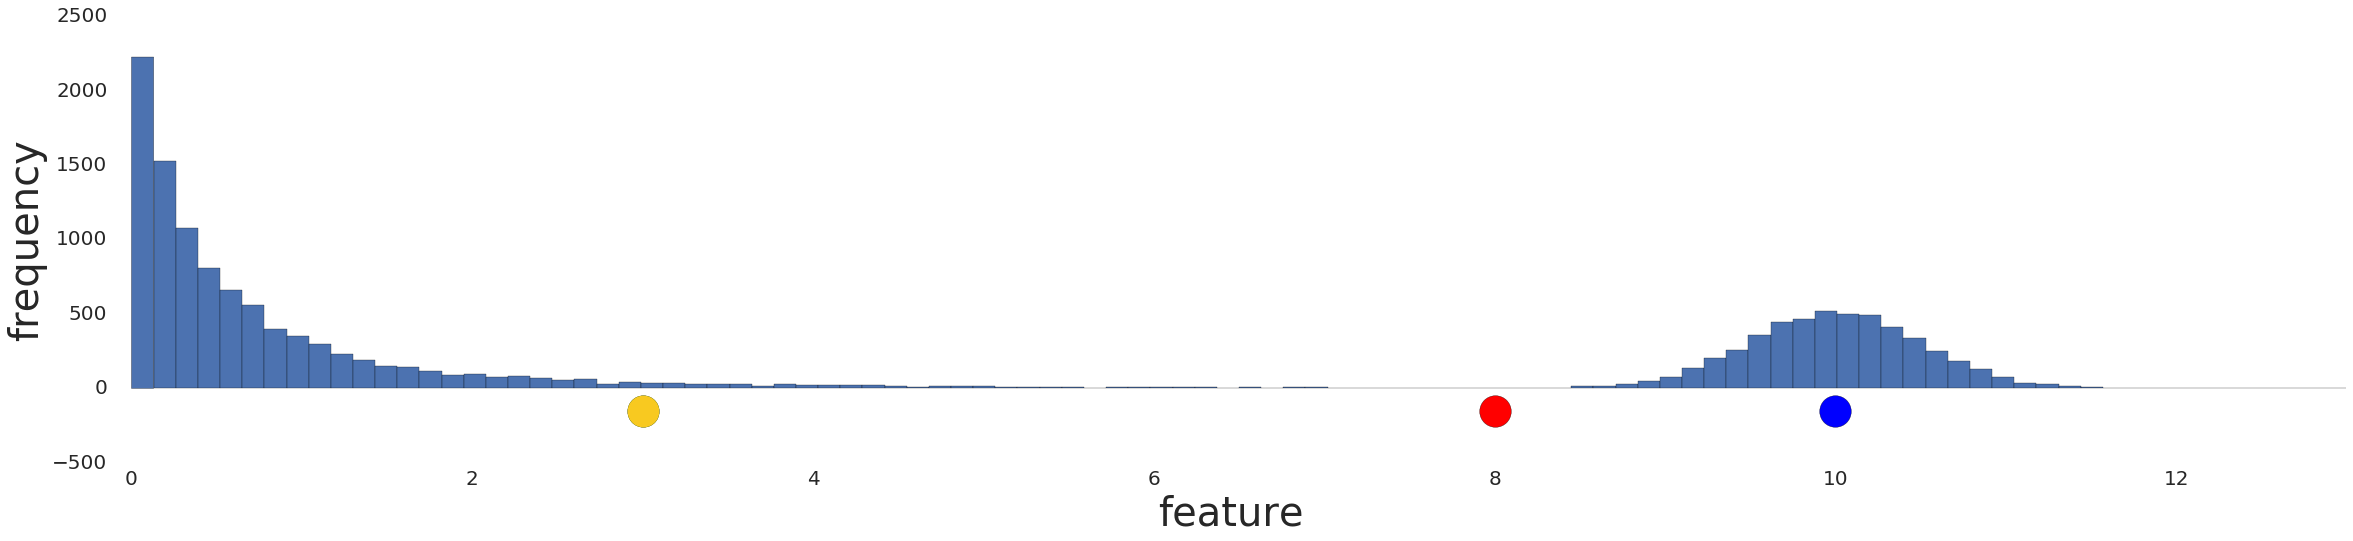
\includegraphics[width=12.0cm]{images/data_prep/scaling_distributions/Preprocess.png}
					\caption{Una distribuzione non categorizzabile, \newline prima di aver applicato un qualunque preprocessing}
		\end{figure}
	%\end{block}
	
\end{frame}


\begin{frame}
	
	\frametitle{{\color{GradientDescentDiagramOrange}Trasformare le distribuzioni}: {\color{GradientDescentDiagramGreen}quantili}}
		
	%\begin{block}{}
		Intuitivamente, se i due esempi hanno solo pochi esempi tra loro, allora questi due esempi sono simili indipendentemente dai loro valori.\\
		Al contrario, se i due esempi hanno molti esempi tra loro, i due esempi sono meno simili.\\
		Pertanto, la \textbf{somiglianza} tra due esempi \textbf{diminuisce all'aumentare del numero di esempi tra di loro}.
		\newlinedouble
		Nè la normalizzazione (trasformazione lineare), nè una log-transform (in figura) riflettono questa intuizione sul funzionamento della somiglianza.
		\begin{figure}[!htbp]
			\centering
			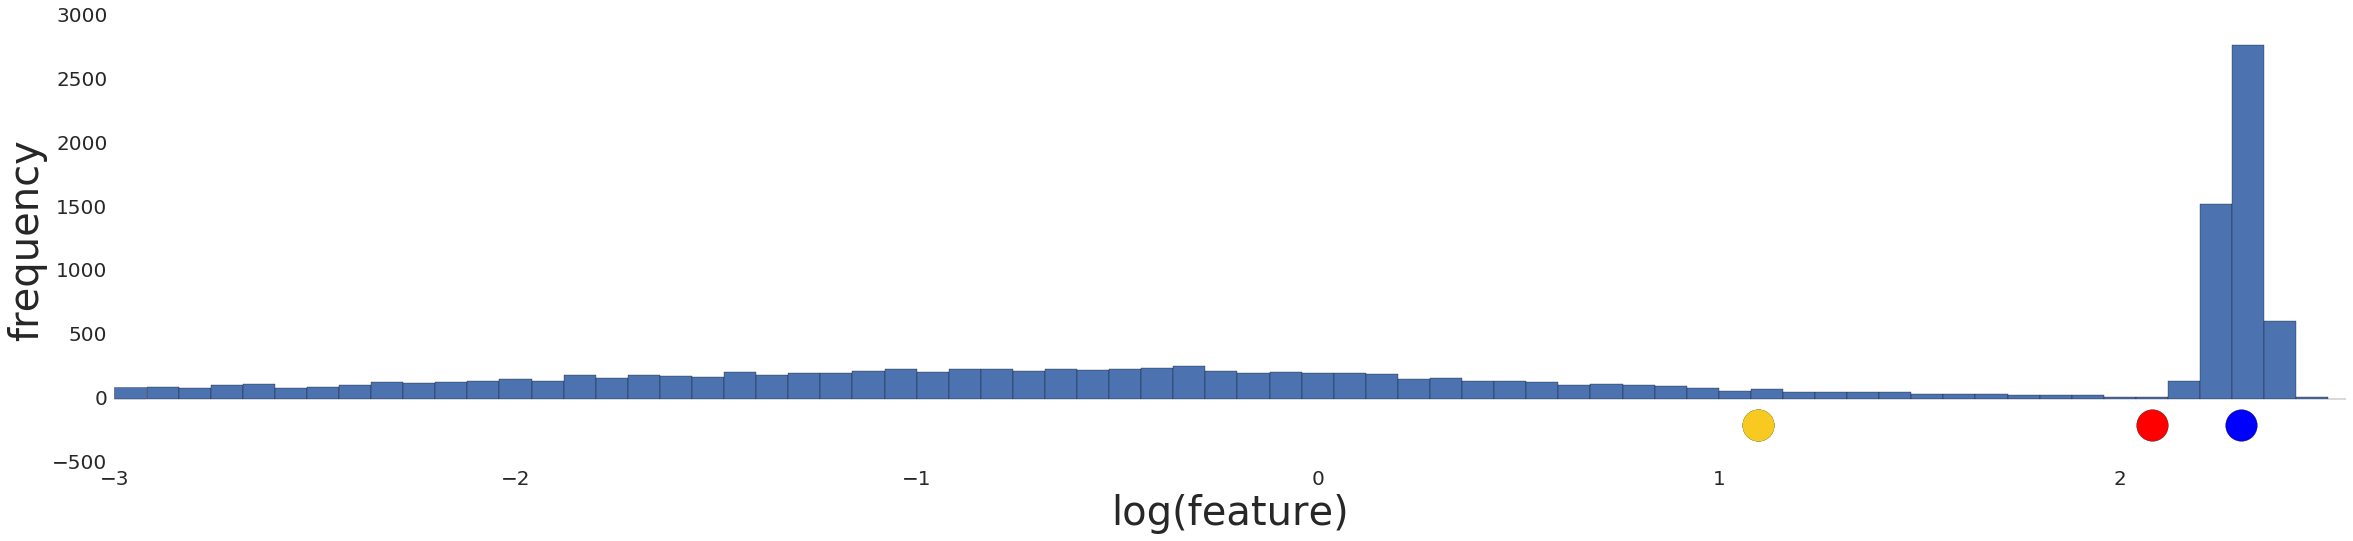
\includegraphics[width=12.0cm]{images/data_prep/scaling_distributions/LogTransform.png}
					%\caption{Dopo aver applicato una log-transform}
		\end{figure}
	%\end{block}
	
\end{frame}


\begin{frame}
	
	\frametitle{{\color{GradientDescentDiagramOrange}Trasformare le distribuzioni}: {\color{GradientDescentDiagramGreen}quantili}}
		
	%\begin{block}{}
		Dividi i dati in intervalli, all'interno del quale ogni intervallo contiene un numero uguale di esempi.
		Questi confini degli intervalli sono detti \textbf{quantili}.\\
		Converti i tuoi dati in quantili eseguendo i seguenti passaggi:
		
		\begin{itemize}
			\item decidi il numero di intervalli
			\item definisci gli intervalli in modo tale che ogni intervallo abbia un numero uguale di esempi
			\item sostituisci ogni esempio con l'indice dell'intervallo al quale appartiene
			\item riporta gli indici allo stesso intervallo dei dati degli altri elementi scalando i valori dell'indice tra [0,1]
		\end{itemize}
		
		\begin{figure}[!htbp]
			\centering
			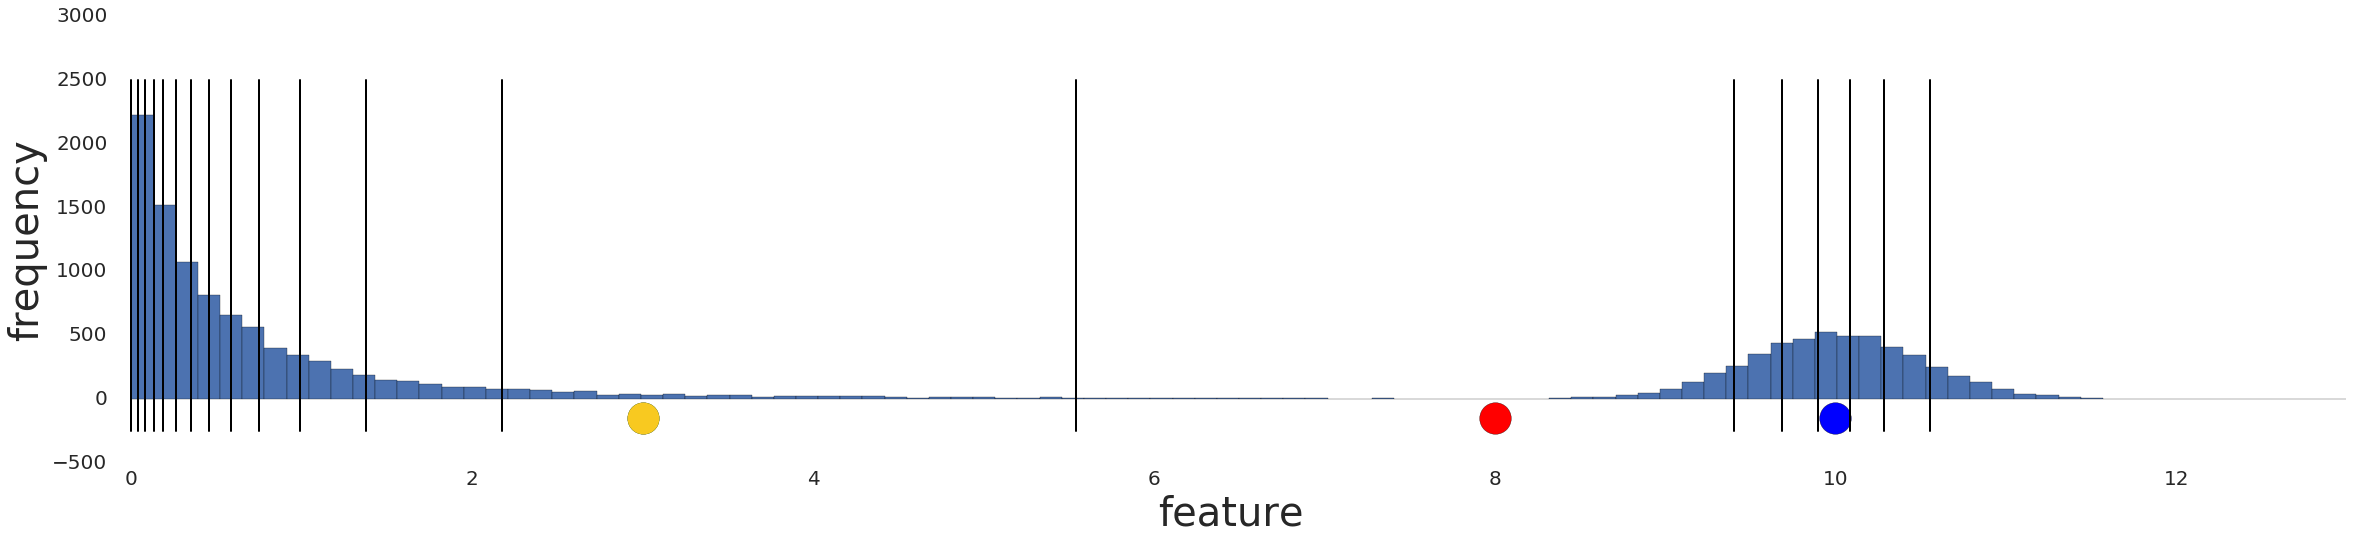
\includegraphics[width=12.0cm]{images/data_prep/scaling_distributions/Quantize.png}
					%\caption{Stripe Radar for Fraud Detection}
		\end{figure}
	%\end{block}
	
\end{frame}



\begin{frame}
	
	\frametitle{{\color{GradientDescentDiagramOrange}Trasformare le distribuzioni}: {\color{GradientDescentDiagramGreen}quantili}}
		
	%\begin{block}{}
		Dopo aver convertito i dati in quantili, la somiglianza tra due esempi è inversamente proporzionale al numero di esempi tra questi due esempi.
		\newlinedouble
		Oppure, matematicamente, dove se per $x$ intendiamo un qualsiasi esempio nel dataset: 
		\begin{itemize}
			\item $sim(A,B) \approx 1 - | \text{prob}[x > A] - \text{prob}[x > B] |$
			\item $sim(A,B) \approx 1 - | \text{quantile}(A) - \text{quantile}(B) |$
		\end{itemize}
		
		 I quantili sono la migliore scelta di default per trasformare i dati.\\
		 Tuttavia, per creare quantili che siano indicatori \textbf{affidabili} della distribuzione dei dati sottostanti, sono necessari \textbf{molti dati}.
		 \newlinedouble
		 Come regola pratica, per creare $n$ quantili, dovresti avere almeno $10n$ esempi. Se non disponi di dati sufficienti meglio applicare una semplice normalizzazione.
	%\end{block}
	
\end{frame}
